\documentclass[journal]{IEEEtran}
\usepackage[a5paper, margin=10mm]{geometry}
%\usepackage{lmodern} % Ensure lmodern is loaded for pdflatex
\usepackage{tfrupee} % Include tfrupee package


\setlength{\headheight}{1cm} % Set the height of the header box
\setlength{\headsep}{0mm}     % Set the distance between the header box and the top of the text


%\usepackage[a5paper, top=10mm, bottom=10mm, left=10mm, right=10mm]{geometry}

%
\usepackage{gvv-book}
\usepackage{gvv}
\usepackage{tikz}
\usepackage{pgfplots}
\pgfplotsset{compat=1.17}
\setlength{\intextsep}{10pt} % Space between text and floats

\makeindex

\begin{document}
\bibliographystyle{IEEEtran}
\onecolumn
\title{
%	\logo{
GATE ASSIGNMENT 4

\large{EE1030 : Matrix Theory}

Indian Institute of Technology Hyderabad
%	}
}
\author{Yellanki Siddhanth

(EE24BTECH11059)
}	


%code by ysiddhanth


\maketitle





\bigskip

\renewcommand{\thefigure}{\theenumi}
\renewcommand{\thetable}{\theenumi}
 
    
        \textbf{2018 CE 53 to 65}\\
\begin{enumerate}
    %code by ysiddhanth 
	\item{
		A waste activated sludge (WAS) is to be blended with green waste (GW). The carbon (C) and nitrogen (N) contents, per kg of WAS and GW, on dry basis are given in the table.
		\begin{center}
		\begin{tabular}{|c|c|c|}
			\hline
			Parameter & WAS & GW \\ \hline
			Carbon (g) & 54 & 360 \\ \hline
			Nitrogen (g) & 10 & 6 \\
			\hline
		\end{tabular}
		\end{center}
		The ratio of WAS to GW required (up to two decimal places) to achieve a blended C:N ratio of 20:1 on dry basis is \underline{\hspace{1.5cm}}
	}
   	\item{
    	Given the following data: design life \( n = 15 \) years, lane distribution factor \( D = 0.75 \), annual rate of growth of commercial vehicles \( r = 6\% \), vehicle damage factor \( F = 4 \) and initial traffic in the year of completion of construction \( = 3000 \) Commercial Vehicles Per Day (CVPD). As per IRC:37-2012, the design traffic in terms of cumulative number of standard axles (in million standard axles, up to two decimal places) is \underline{\hspace{1.5cm}}
    }
    \item{
            An aircraft approaches the threshold of a runway strip at a speed of 200 km/h. The pilot decelerates the aircraft at a rate of \(1.697 \, m/s^2\) and takes 18 s to exit the runway strip. If the deceleration after exiting the runway is \(1 \, m/s^2\), then the distance (in m, up to one decimal place) of the gate position from the location of exit on the runway \underline{\hspace{1.5cm}}
        }
    \item[]{
    \textbf{Q. 1 – Q. 5 carry one mark each.}}
	\item{
        	
        	“His face \( \underline{\hspace{2cm}} \) with joy when the solution of the puzzle was \( \underline{\hspace{2cm}} \) to him.”
        	The words that best fill the blanks in the above sentence are
        	\begin{enumerate}
        		\begin{multicols}{2}
        			\item shone, shown
        			\item shone, shone
        			\item shown, shone
        			\item shown, shown
        		\end{multicols}
        	\end{enumerate}
        	
      }
        \item {“Although it does contain some pioneering ideas, one would hardly characterize the work
        	as \( \underline{\hspace{2cm}} \).”
        	The word that best fills the blank in the above sentence is
        	\begin{enumerate}
        		\begin{multicols}{4}
        			\item innovative
        			\item simple
        			\item dull
        			\item boring
        		\end{multicols}
        	\end{enumerate}
  		}
    
    \item {
    	\(\underbrace{a + a + a + \dots + a}_{n \text{ times}} = a^2 b\) and \(\underbrace{b + b + b + \dots + b}_{m \text{ times}} = a b^2\), where \(a\), \(b\), \(n\) and \(m\) are natural numbers. What is the value of \((\underbrace{m + m + m + \dots + m}_{n \text{ times}}) (\underbrace{n + n + n + \dots + n}_{m \text{ times}})\)?
    	\begin{multicols}{4}
	    	\begin{enumerate}
	    		\item \(2a^2b^2\)
	    		\item \(a^4b^4\) 
	    		\item\(ab(a+b)\) 
	    		\item \(a^2 + b^2\) 
	    	\end{enumerate}
    	\end{multicols}
    
    }    
    \item {A three-member committee has to be formed from a group of 9 people. How many such distinct committees can be formed?
    	\begin{multicols}{4}
	    	\begin{enumerate}
	    		\item 27
	    		\item 72
	    		\item 81
	    		\item 84
	    	\end{enumerate}
    	\end{multicols}}
    \item {For non-negative integers \(a\), \(b\), \(c\), what would be the value of \(a + b + c\) if \(\log a + \log b + \log c = 0\)?
    	\begin{multicols}{4}
    		\begin{enumerate}
    			\item 3
    			\item 1
    			\item 0
    			\item $-1$
    		\end{enumerate}
    	\end{multicols}
	}
	\item[]{\textbf{Q. 6 – Q. 10 carry two marks each}}
    \item {
    	In manufacturing industries, loss is usually taken to be proportional to the square of the deviation from a target. If the loss is Rs. 4900 for a deviation of 7 units, what would be the loss in Rupees for a deviation of 4 units from the target?
    	
    	
    	\begin{multicols}{4}
    		\begin{enumerate}
    			\item 400 
    			\item 1200 
    			\item 1600
    			\item 2800
    		\end{enumerate}
    	\end{multicols}
    
	}
    \item{
            A faulty wall clock is known to gain 15 minutes every 24 hours. It is synchronized to the correct time at 9 AM on 11th July. What will be the correct time to the nearest minute when the clock shows 2 PM on 15th July of the same year?
            
            
                
            \begin{multicols}{4}
                \begin{enumerate}
                	\item 12:45 PM 
                	\item 12:58 PM
                	\item 1:00 PM
                	\item 2:00 PM
                \end{enumerate}
            \end{multicols}

        %code by ysiddhanth 
        
        }
    \item{
            The annual average rainfall in a tropical city is 1000 mm. On a particular rainy day (24-hour period), the cumulative rainfall experienced by the city is shown in the graph. Over the 24-hour period, 50\% of the rainfall falling on a rooftop, which had an obstruction-free area of 50 m$^2$, was harvested into a tank. What is the total volume of water collected in the tank in liters?
          \begin{center}
          	\begin{tikzpicture}
          		\begin{axis}[
          			width=6cm, height=6cm,
          			xlabel={Hours},
          			ylabel={Cumulative rainfall (mm)},
          			xmin=0, xmax=24,
          			ymin=0, ymax=400,
          			xtick={0,3,6,9,12,15,18,21,24},
          			ytick={0,50,100,150,200,250,300,350,400},
          			grid=both,
          			major grid style={line width=.2pt,draw=gray!50},
          			minor grid style={line width=.1pt,draw=gray!20},
          			thick
          			]
          			\addplot[mark=none, black] coordinates {
          				(0, 0) (9, 100) (12, 200) (15, 200) (18, 300) (21, 300) (24, 300)
          			};
          		\end{axis}
          	\end{tikzpicture}
          \end{center}
            \begin{enumerate}
            	\begin{multicols}{4}
            		\item 25,000
            		\item 18,750
            		\item 7,500
            		\item 3,125
            	\end{multicols}
            \end{enumerate}
        
        }
    \item{
            Given that \( \frac{\log P}{y-z} = \frac{\log Q}{z-x} = \frac{\log R}{x-y} = 10 \) for \( x \ne y \ne z \), what is the value of the product \( PQR \)?
            \begin{enumerate}
            	\begin{multicols}{4}
            		\item (A) 0
            		\item (B) 1
            		\item (C) $xyz$
            		\item (D) $10^{xyz}$
            	\end{multicols}
            \end{enumerate}
        }
    \item{
        
           	Each of the letters in the figure below represents a unique integer from 1 to 9. The letters are positioned in the figure such that each of \((A+B+C)\), \((C+D+E)\), \((E+F+G)\) and \((G+H+K)\) is equal to 13. Which integer does \(E\) represent?
           	\begin{center}
           		\begin{tikzpicture}
           			% Define block style
           			\tikzstyle{block} = [draw, minimum width=1cm, minimum height=1cm]
           			
           			% Draw blocks with letters
           			\node[block] (A) at (0,0) {A};
           			\node[block] (B) at (1,0) {B};
           			\node[block] (C) at (2,0) {C};
           			
           			\node[block] (D) at (2,-1) {D};
           			
           			\node[block] (E) at (2,-2) {E};
           			\node[block] (F) at (3,-2) {F};
           			\node[block] (G) at (4,-2) {G};
           			
           			\node[block] (H) at (4,-3) {H};
           			\node[block] (K) at (4,-4) {K};
           		\end{tikzpicture}
           	\end{center}
           	\begin{multicols}{4}
           		
				\begin{enumerate}
					\item 1
					\item 4
					\item 6
					\item 7
				\end{enumerate}
			\end{multicols}

        
        }
   
    \end{enumerate}
\end{document}



